The WDN of concern in this paper is a two-pump, two-consumer, single-EWR system as seen on \cref{fig:WDNModel}.

\begin{figure}[h]
	\centering
	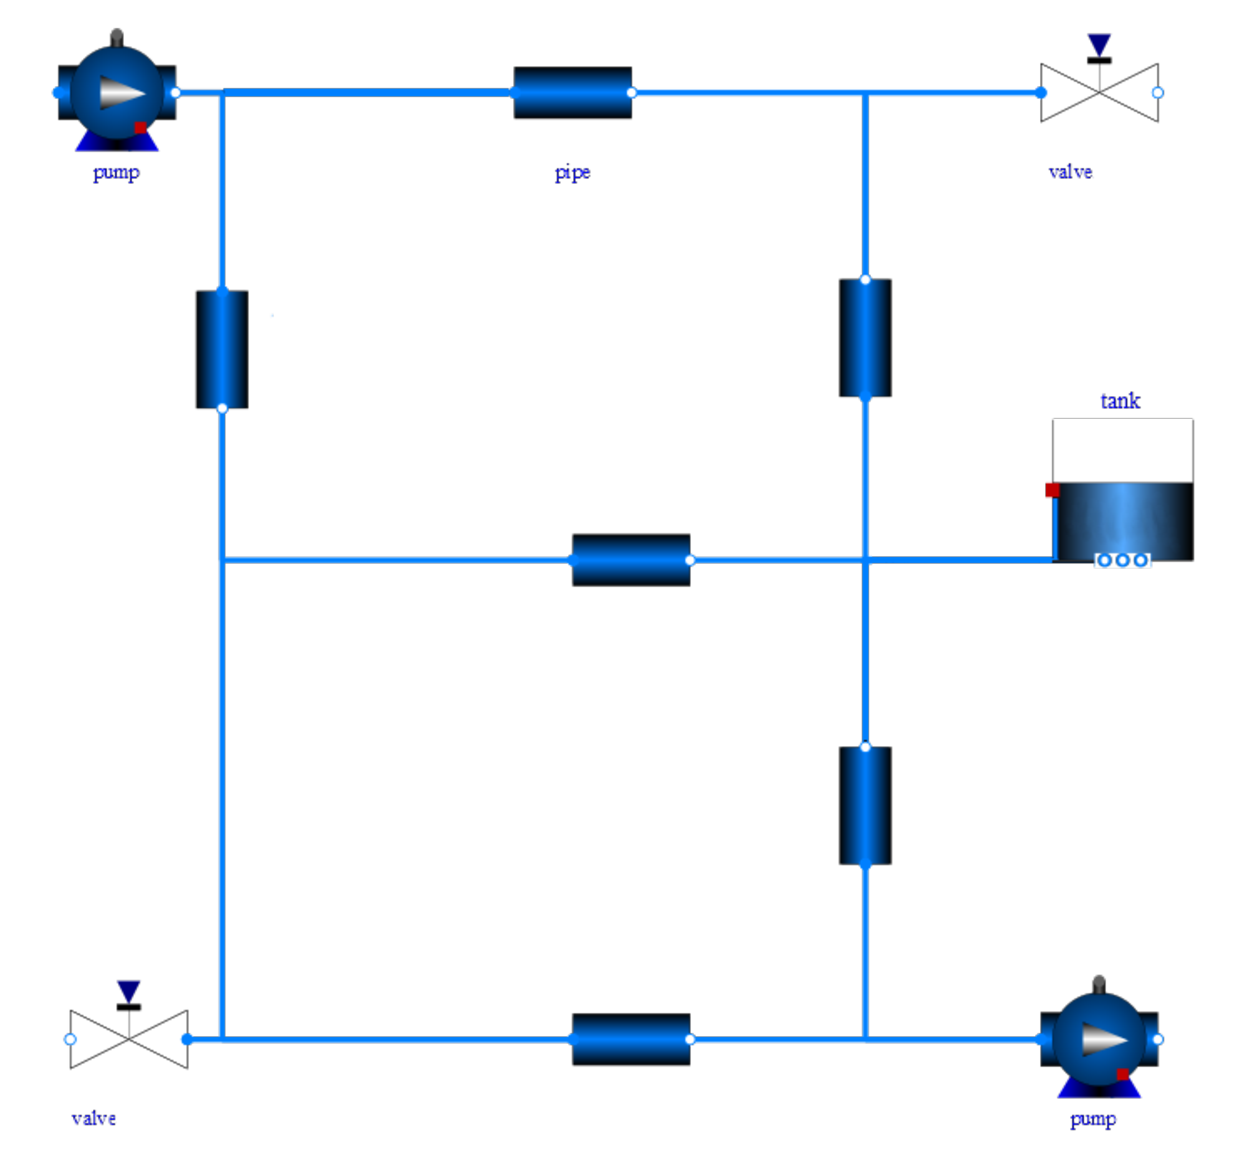
\includegraphics[width=0.5\linewidth]{Graphics/WDNModel.pdf}
	\caption{Schematic of the WDN under study.}
	\label{fig:WDNModel}
\end{figure}

As described in \Cref{sec:Introduction}, the dynamics of a WDN can be separated into a tank slow pressure regime and a fast flow regime. We use a directed graph model of the WDN corresponding to \cref{fig:tikzWDNGraph}, with the vertices $\{v_1,..,v_n\}$, edges $\{e_1,..,e_m\}$, nodal demands and nodal heights $d_i, h_i$ and edge flows $q_i$:

\begin{figure}[h!]
	\centering
	\resizebox{\columnwidth}{!}{
			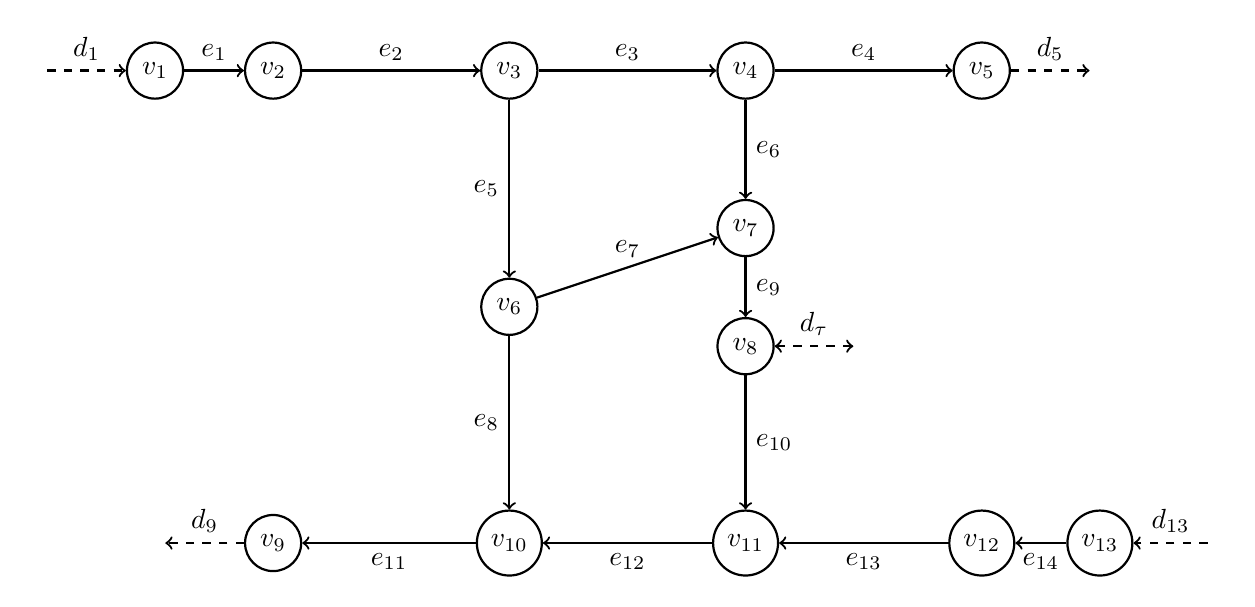
\begin{tikzpicture}[node distance=30mm, thick, main/.style = {draw,circle}] 
		\node (1)  {};
		\node[main] (2) [node distance={15mm},right of=1] {$v_1$}; 
		\node[main] (3) [node distance={1.5cm},right of=2] {$v_2$};
		\node[main] (4) [right of=3] {$v_3$};
		\node[main] (5) [right of=4] {$v_4$};
		\node[main] (6) [right of=5] {$v_5$};
		\node (7) [node distance={15mm},right of=6] {};
		%Create 3 (4) nodes in middle part of graph
		\node[main] (8) [below of=4] {$ v_6 $};
		\node[main] (9) [node distance={20mm},below of=5] {$ v_7 $};
		\node[main] (11) [node distance={15mm},below of=9] {$ v_8 $};
		\node (10) [node distance={15mm},right of=11] {};
		%First 5 (7) nodes in bottom part of graph
		\node[main] (12) [below of=8] {$ v_{10} $};
		\node[main] (13) [left of=12] {$ v_9 $};
		\node(14) [node distance={15mm},left of=13] {};
		\node[main] (15) [right of=12] {$ v_{11} $};
		\node[main] (16) [right of=15] {$ v_{12} $};
		\node[main] (17) [node distance={1.5cm},right of=16] {$ v_{13} $};
		\node(18) [node distance={15mm},right of=17] {};
		
		%Edges with direction
		\path [->] (2) edge node[above] {$e_{1}$} (3); 	%Edge v1 -> v2
		\path [->] (3) edge node[above] {$e_{2}$} (4); 	%Edge v2 -> v3
		\path [->] (4) edge node[above] {$e_{3}$} (5); 	%Edge v3 -> v4
		\path [->] (5) edge node[above] {$e_{4}$} (6); 	%Edge v4 -> v5
		
		\path [->] (4) edge node[left] {$e_{5}$} (8); 	%Edge v3 -> v6
		\path [->] (5) edge node[right] {$e_{6}$} (9); 	%Edge v4 -> v7
		\path [->] (8) edge node[above] {$e_{7}$} (9); 	%Edge v6 -> v7
		\path [->] (8) edge node[left] {$e_{8}$} (12); 	%Edge v6 -> v10
		\path [->] (9) edge node[right] {$e_{9}$} (11); 	%Edge v7 -> v8
		\path [->] (11) edge node[right] {$e_{10}$} (15);	 %Edge v8 -> v11
		
		
		\path [->] (12) edge node[below] {$e_{11}$} (13); %Edge v10 -> v9
		\path [->] (15) edge node[below] {$e_{12}$} (12); %Edge v11 -> v10
		\path [->] (16) edge node[below] {$e_{13}$} (15); %Edge v12 -> v11
		\path [->] (17) edge node[below] {$e_{14}$} (16); %Edge v13 -> v12
		
		%External flows
		\draw[->,dashed,] (1) -- node[above] {$d_1$} (2); %Create d1
		\draw[->,dashed,] (6) -- node[above] {$d_5$} (7); %Create d5
		\draw[->,dashed,] (13) -- node[above] {$d_9$} (14); %Create d13
		\draw[->,dashed,] (18) -- node[above] {$d_{13}$} (17); %Create d13
		\draw[<->,dashed,] (10) -- node[above] {$d_\tau$} (11); %Create d_tau
	\end{tikzpicture} }
		\caption{Graph Network of Water Distributed Network. Note that $e_1$ and $e_{14} $ are only inserted to be able to measure pump flow.}
	\label{fig:tikzWDNGraph}
\end{figure}  

Applying standard graph theory - see e.g. Deo \cite{Deo} - we obtain an incidence matrix $H$ and loop matrix $B$ with the chords $E_C=\{e_3,e_7\}$ chosen. We furthermore introduce the notation $H_T$ for the columns of $H$ in the spanning tree $E_T=\{e_1,e_2,e_4,..,e_6,e_8,..,e_{14}\}$, while $H_C$ is given by the columns of $H$ in $E_C=\{e_3,e_7\}$. The reduced incidence matrix $\bar{H}$ is obtained by choosing the node $ v_{13} $ as reference and eliminating the corresponding row of $H$.

In addition to these graph-related definitions, we require boundary conditions imposed by Kirchhoff's laws, which for an open WDN are given \cite{Jensen} by:
\begin{gather}
	Hq = d \label{eq:KirchNodeLaw} \\
	B\Delta p = B H^T p = 0 \wedge B\Delta h = B H^T h = 0 \label{eq:KirchMeshLaw}
\end{gather} 

Where $p$ is the vector of nodal pressures. Furthermore, mass conservation is assumed at the graph boundary. This implies that there can at most be $n-1$ independent nodal demands, i.e.:

\begin{equation}\label{eq:MassConservation}
	d_n = -\sum_{i=1}^{n-1}d_i
\end{equation}

%Secondly, we require two lemmas pertaining to the spanning tree subspace $H_T$ of $H$: \\
%
%\begin{lem}\label{lem:TreePartitionLemma}
%	Let $H_T$ be the incidence matrix partition corresponding to the spanning tree of the graph described by $H$, and let $\bar{H}_T$ be its equivalent with respect to the reduced incidence matrix $\bar{H}$. $\bar{H}_T$ is invertible since a tree is a connected graph with $n-1$ edges \cite{Deo}, and the following holds:
%	
%	\begin{equation}\label{eq:TreePartitionLemma}
%		H_T\bar{H}_T^{-1} = \begin{bmatrix} I_{n-1} \\ \mathbbm{1}^T	\end{bmatrix}
%	\end{equation}
%	
%	where $\mathbbm{1}$ is a vector of ones and $I_{n-1} \in \mathbb{R}^{n-1 \times n-1}$ is an identity matrix.
%\end{lem}
%
%\newpage
%
%\begin{lem}\label{lem:EdgeFlowDecomposition}
%	Let $q \in \mathbb{R}^m$ be the edge flows of a graph with reduced incidence matrix $\bar{H}$ and $n$ nodes. Denote its spanning tree by $T$, let $q_c \in \mathbb{R}^c, \ c = m-n+1$ be the graph's chordal flows, and denote the tree partition of the reduced incidence matrix $\bar{H}_T$. Finally, let $B$ be the graph's fundamental loop matrix, and define $\bar{d} \in \mathbb{R}^{n-1}$ as the vector of non-reference nodal demands. Then the following is true:
%	
%	\begin{equation}\label{eq:EdgeFlowDecomposition}
%		q = B^T q_c +
%		\begin{bmatrix}
%			0_{c \times n-1} \\ \bar{H}_T^{-1} 
%		\end{bmatrix}
%		\bar{d}
%	\end{equation}
%\end{lem}
%
%With these definitions in hand, we move on to modelling of the slow dynamics.

\subsection{Slow Dynamics}\label{subsec:SlowDynamics}

The evolution of pressure $p_\tau$ in an EWR, assuming only one tank orifice, and defining the positive flow direction as \textit{from} the tank, can be described \cite{Kallesoe2017} by the equation:

\begin{gather}\label{eq:TankPressureDyn}
	\dot{p}_\tau = -\tau d_\tau
	\\ \tau = \rho g \frac{1}{A_\tau}
\end{gather}

where $\rho$ is the density of the working fluid, $g$ is gravitational acceleration, and $A_\tau$ is the cross-sectional area of the tank. This can be discretised by Euler's method such that:

\begin{equation}\label{eq:DiscreteTankPressureDyn}
	p_\tau(k+1) = p_\tau(k) - \tau d_\tau(k)t_s =  p_\tau(k) - \mathcal{T} d_\tau(k)
\end{equation}

Now by the mass conservation condition in \cref{eq:MassConservation}, we can rewrite \cref{eq:DiscreteTankPressureDyn} in terms of the other flows at the system boundary:

\begin{equation}\label{eq:DiscreteTankPressureDynConProd}
	p_\tau(k+1) = p_\tau(k) - \mathcal{T} d_\tau(k) = p_\tau(k) + \mathcal{T} \Big(d_p(k) + d_c(k)\Big)
\end{equation}

which can be represented as a discrete state-space model with a disturbance term:

\begin{equation}\label{eq:DiscreteTankPressureStateSpace}
	\begin{gathered}
	p_\tau(k+1) = Ap_\tau(k) + B_p d_p(k) + B_cd_c(k) \\ B_p = B_c = \begin{bmatrix}\mathcal{T} & \mathcal{T} \end{bmatrix}
	\end{gathered}
\end{equation}

We note that the consumer flows $d_c$ can be considered a disturbance to be cancelled under this interpretation, while the pump flows $d_p$ can be considered the input to the pressure dynamics. This supports the concept of an inner flow control loop and a disturbance rejection scheme.

\subsection{Fast Dynamics}\label{subsec:FastDynamics}

In contrast to the slow dynamics, which are effected exclusively by the mass conservation boundary condition, the fast dynamics of the WDN are effected by the behaviour on each individual edge in conjunction with the boundary conditions. A general function for the behaviour on an arbitrary WDN edge is given by \cite{Jensen}:

\begin{equation}\label{eq:GeneralEdgeModel}
	\Delta p = \mathcal{J}\dot{q} + \lambda(q) + \mu(q,\Theta) + \alpha(q,\omega) + \Delta z
\end{equation}

where $\mathcal{J},\lambda$ apply only to pipes, $\mu$ applies only to valves, $\alpha$ applies only to pumps, and $\Delta z$ is the pressure change induced by height difference along the edge traverse. $q,\Theta,\omega$ are respectively the flow, valve opening degree, and pump rotational speed at the edge in question. We refer to \cite{Swamee2008,KallesoePhD} for a detailed breakdown of each component model.

%\textbf{Pipe Model:}
%The differential pressure across the $ k^{th} $ pipe is modelled as:
%\begin{equation}\label{eq:PipeModel}
%	\begin{gathered}
%		\Delta{p_{k}} = \mathcal{J}_k\dot{q}_k + \lambda(q_k) + \Delta z_k \\ 
%		\mathcal{J}_k = \frac{L_k\cdot \rho}{A_k} \\
%		\mathcal{\lambda}(q_k) = \left(f \cdot \frac{8\cdot L_k \cdot \rho}{\pi^{2} \cdot D_k^{5}} + k_{f}\cdot \frac{8\cdot \rho}{\pi^{2} \cdot D_k^{4}}\right)\cdot |q_{k}|\cdot q_{k}\\
%		\Delta z_k = - \rho \cdot g \cdot \Delta{h_{k}}
%	\end{gathered}
%\end{equation}
%
%where $L_k, D_k$ are the length and diameter of the $k$th pipe, while $f,k_f$ are the pipe friction and form loss factors as given in \cite{Swamee2008}.
%
%\textbf{Valve Model:}
%The differential pressure across the $ k^{th} $ valve, assuming a linear-type \cite{Swamee2008}, is given by:
%\begin{equation}\label{eq:ValveModel}
%	\begin{gathered}
%		\Delta p_{k} = \mu_k(q_k,\Theta) \\ 
%		\mu_k(q_k,\Theta) = \frac{1}{K_{valve}(\Theta)^2} \cdot |q_k|\cdot q_k
%	\end{gathered}
%\end{equation}
%
%\textbf{Pump Model:}
%The differential pressure across the $ k^{th} $ pump is modelled as:
%\begin{equation}\label{eq:PumpPressure}
%	\begin{gathered}
%		\Delta p_{k} =   \alpha(q_k,\omega_k) \\
%		\alpha(q_k,\omega_k) = a_0\cdot \omega_k^2 +  a_1\cdot \omega_k \cdot q_k -a_2\cdot |q_k|\cdot q_k
%	\end{gathered}
%\end{equation}
%Coefficients are found by fitting the pump curves in \cite{GrundfosDatablad}. In practice we neglect the $ a_1 $ cross term to simplify analysis.

%\begin{table}[thpb]\label{tab:PumpCoeffs}
%	\centering
%	\begin{tabular}{cc}
%		\toprule
%		Coefficient & Value  \\ \toprule
%		$a_0$  &   $0.0001$   \\ 
%		$a_1$  &   $0.0004$   \\
%		$a_2$  &   $-0.0323$  \\ \bottomrule
%	\end{tabular}
%	%	\caption{Pump Coefficients for Grundfos UPM3(K) pump}
%	\label{tab:PumpCoeff}
%\end{table}


We now introduce the open-node and tank mapping matrices ${F}$ and ${G}$, which are defined such that the edge flows can be written as:

\begin{equation}\label{eq:FlowDecomposition}
		q = B^T q_c +	\begin{bmatrix} 0_{c \times n-1} \\ {H}_T^{-1} \end{bmatrix}\Big({F}d_f + {G}d_\tau \Big)
\end{equation}

where $q_c$ are the flows in the chords, $d_f$ is the vertex-ordered vector of non-tank demands at the boundary, and $d_\tau$ is the vector of tank demands at the boundary. We can then state the full nonlinear model of the fast dynamics as \cite{Rathore1030,Jensen}:




%We can then use the boundary condition \cref{eq:KirchMeshLaw} to obtain:
%
%\begin{equation}\label{eq:ChordEquations}
%	B\mathcal{J}\dot{q} = -B(\lambda(q) + \mu(q,\Theta) + \alpha(q,\omega))
%\end{equation}
%
%and by invoking the boundary condition \cref{eq:KirchNodeLaw} and \cref{lem:TreePartitionLemma}, we can rewrite this exclusively as a function of the flows at the boundary and the chord flows:
%
%\begin{equation}\label{eq:ChordEquationsSimple}
%	\begin{split}
%	B\mathcal{J}B^T\dot{q}_C &-\bar{H}_C^T\bar{H}_T^{-T}\mathcal{J}_T\bar{H}_T^{-1} \bar{F} \dot{d_f} \\
%	&-\bar{H}_C^T\bar{H}_T^{-T}\mathcal{J}_T\bar{H}_T^{-1} \bar{G} \dot{d_{\tau}} \\
%	&= -B(\lambda(q) + \mu(q,\Theta) + \alpha(q,\omega))
%	\end{split}
%\end{equation}
%
%We now address the spanning tree, where the following identity holds:
%
%\begin{equation}\label{eq:SpanTPressures}
%	\begin{split}
%		H_T^T \begin{bmatrix} \bar{p} \\ p_0	\end{bmatrix} = 
%		\mathcal{J}_T\dot{q}_T &+ (\lambda_T(q_T)+\mu_T(q_T) + \alpha_T(q_T)) \\ 
%		&-H_T^T \begin{bmatrix} \bar{z} \\ z_0	\end{bmatrix}
%	\end{split}
%\end{equation}
%
%Assuming a reference node at atmospheric pressure is chosen, and addressing first the non-tank boundary flows, \cref{lem:TreePartitionLemma} and \cref{eq:KirchNodeLaw} can be leveraged to rewrite \cref{eq:SpanTPressures} as:
%
%\begin{equation}\label{eq:SpanTBoundaryFlows}
%	\begin{split}
%	-\bar{F}^T\bar{H}_T^{-T}\mathcal{J}_T\bar{H}_T^{-1}\bar{H}_C\dot{q}_C + \bar{F}^T\bar{H}_T^{-T}\mathcal{J}_T\bar{H}_T^{-1}\bar{F}\dot{d}_f \\ 
%	+ \bar{F}^T\bar{H}_T^{-T}\mathcal{J}_T\bar{H}_T^{-1}\bar{G}\dot{d}_{\tau} \\
%	= -\bar{F}^T\bar{H}_T^{-T}(\lambda_T(q_T)+\mu_T(q_T,\Theta) + \alpha_T(q_T,\omega)) \\
%	+\bar{F}^T(\bar{z} - \mathbf{1}z_0)
%\end{split}
%\end{equation}
%
%as pathing from one open node to another must inherently result in no net pressure change. A similar equation can be written considering the boundary flow at the tank:
%
%\begin{equation}\label{eq:SpanTTankFlows}
%	\begin{split}
%	-\bar{G}^T\bar{H}_T^{-T}\mathcal{J}_T\bar{H}_T^{-1}\bar{H}_C\dot{q}_C + \bar{G}^T\bar{H}_T^{-T}\mathcal{J}_T\bar{H}_T^{-1}\bar{F}\dot{d}_f \\
%	+ \bar{G}^T\bar{H}_T^{-T}\mathcal{J}_T\bar{H}_T^{-1}\bar{G}\dot{d}_{\tau} \\
%	= -\bar{G}^T\bar{H}_T^{-T}(\lambda_T(q_T)+\mu_T(q_T,\Theta) + \alpha_T(q_T,\omega)) \\
%	+ \bar{G}^T(\bar{z} - \mathbf{1}z_0) +	(\bar{p}_\tau - \mathbf{1}p_0) \\	
%\end{split}
%\end{equation}

%These three equations \cref{eq:ChordEquationsSimple,eq:SpanTBoundaryFlows,eq:SpanTTankFlows} then define the entire fast dynamics of the WDN, and can be collected in the following compact form:

\begin{equation}\label{eq:NonLinearModelWithTank}
	\begin{split}
		\Phi\mathcal{J}\Phi^T \dot{q}_n = &-\Phi\Big(\lambda(q_n)+\mu(q_n,\Theta)+\alpha(q_n,\omega)\Big)\\ 
		&+ \Psi(\bar{z}-\mathbf{1}z_0) + \mathcal{I}(p_{\tau}-\mathbf{1}p_0)
	\end{split}
\end{equation}

where $q_n = \{q_c, d_f, d_\tau\}^T$and the matrices $\Phi, \Psi, \mathcal{I}$ are defined as:

\begin{equation}\label{eq:NonLinearModelMatrices}
	\Phi \triangleq 
	\begin{bmatrix} 
		I & -\bar{H}_C^T\bar{H}_T^{-T} \\ 0 & \bar{F}^T\bar{H}_T^{-T} \\ 0  & \bar{G}^T\bar{H}_T^{-T} \\ 
	\end{bmatrix}
	, \quad
	\Psi \triangleq
	\begin{bmatrix}
		0 \\ \bar{F}^T \\ \bar{G}^T
	\end{bmatrix}
	, \quad
	\mathcal{I} \triangleq
	\begin{bmatrix}
		0 \\ 0 \\ I
	\end{bmatrix}
\end{equation}

\subsection{Linearised Model}

The full fast dynamics \cref{eq:NonLinearModelWithTank} are nonlinear with respect to several variables. This makes the model unsuitable for use with the control methods employed in this paper, and a linearisation is therefore necessary. This linearisation is performed by taking the $1$st-order Taylor expansion of \cref{eq:NonLinearModelWithTank} at an equilibrium point $x_0$ such that:

\begin{equation}\label{eq:TaylorSeries}
	\dot{x} \approx f(x_0) + \nabla f\bigg\rvert_{x_0} (x-x_0)
\end{equation}

We note that it can be shown that neglecting $\frac{\partial f}{\partial \Theta}$ and $\frac{\partial f}{\partial p_\tau}$ leads to a constant error at steady-state under the assumption that their dynamics are far slower than $\omega$ and $q$. Thus, \cref{eq:TaylorSeries} can be reduced to:

\begin{equation}\label{eq:TaylorSeriesSimple}
\begin{gathered}
	\dot{q}_n \approx \dfrac{\partial f}{\partial q_n} \tilde{q}_n + \dfrac{\partial f}{\partial \omega} \tilde{\omega} \\
	\tilde{q}_n = q_n-q_0 \wedge \tilde{\omega} = \omega-\omega_0
\end{gathered}
\end{equation}

which exactly fits a classical linear state-space model structure of:

\begin{equation}\label{eq:}
	\begin{gathered}
		\dot{\tilde{q}}_n = A\tilde{q}_n + B \tilde{\omega}_n \\
		\tilde{d}_p = C \tilde{q}_n
	\end{gathered}
\end{equation}

Linearising \cref{eq:NonLinearModelWithTank} at its lone equilibrium point results in the following approximation:

\begin{equation}\label{eq:LinearisedModelWithTank}
\begin{gathered}
	A = \begin{bmatrix}
		-0.35 & -0.03 & 0.00 & 10.21 & -0.77 & 0.00\\
		-0.12 & -0.33 & 0.21 & -1.37 & -6.17  & 0.00\\
		-0.02 & 0.08 & -0.24 & 7.28 & 1.54 & 0.00\\
		0.14 & 0.08 & -0.04 & -20.51 & 1.54 & 0.00\\
		-0.07 & -0.05 & 0.05 & 1.54 & -15.44 &   -0.02\\
		0.15 & 0.10 & -0.08 & 11.57 & 8.64 & -0.10\\
	\end{bmatrix} \\
	B = \begin{bmatrix}
		0.10 & 0.00\\
		0.01 & 0.00 \\
		0.12 & 0.00 \\
		-0.04 & 0.00 \\
		-0.01 & -0.02\\
		-0.07 & -0.07
	\end{bmatrix}
\\
		C = \begin{bmatrix} 
			0 & 0 & 1 & 0 & 0 & 0	\\		
			0 & 0 & -1 & -1 & -1 & -1
		\end{bmatrix}
\end{gathered}
\end{equation}

We note that the eigenvalues of $A$ are strictly negative with nonzero real part, which means that the equilibrium point is stable and hyperbolic \cite{Khalil}, and resultingly by the Hartman-Grobman theorem the linear model is exact in some region around the equilibrium \cite{Perko2001}. This can be confirmed by co-simulation of the full nonlinear model with the linear model as a $1$-step-ahead predictor:


\begin{figure}[h]
	\centering
	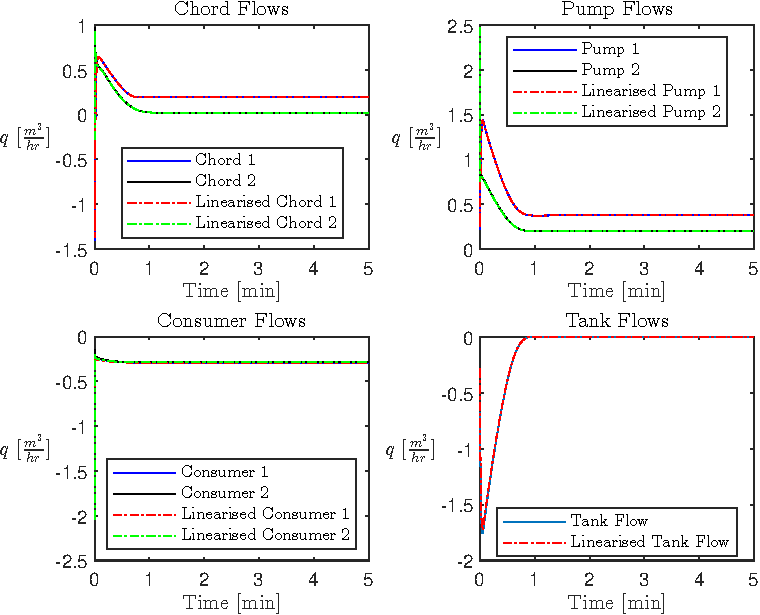
\includegraphics[height = 4cm,width=\linewidth]{Graphics/NominalFlows.pdf}
	\caption{Comparison of nonlinear and linearised model behaviour, $1$-step-ahead prediction at operating point.}
	\label{fig:CompNonLinEQ}
\end{figure}

Evaluating the model away from the linearisation operating point ($\Theta = \{0.7,0.4\} \wedge \omega = \{80,40\}$), we see per \cref{fig:CompNonLinNotEQ} that the model is still largely accurate.

\begin{figure}[h]
	\centering
	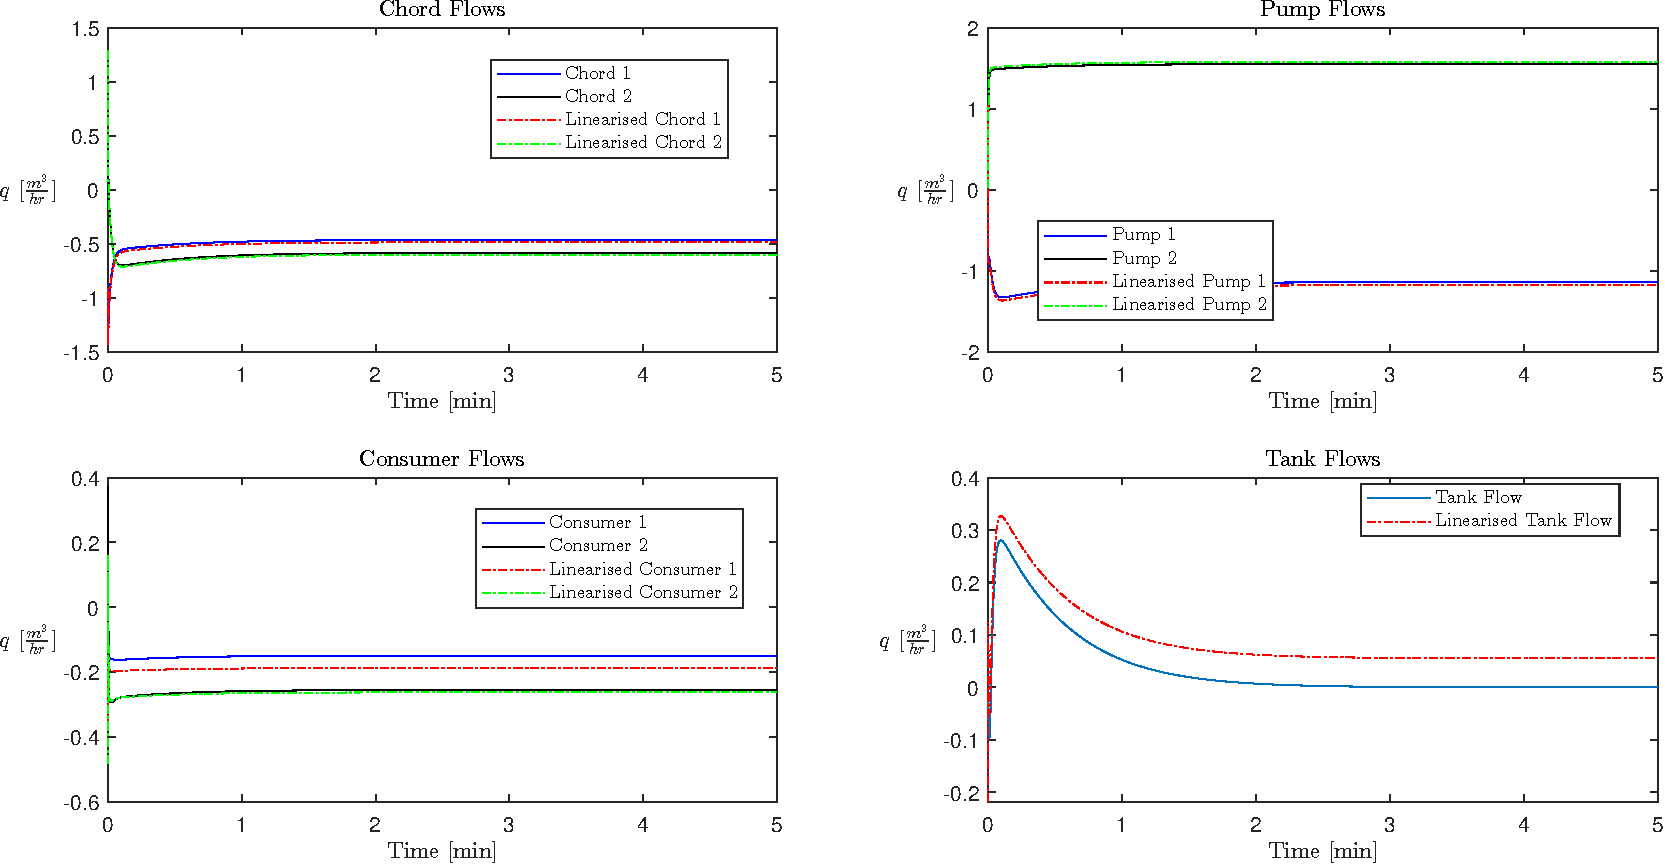
\includegraphics[height=4cm,width=\linewidth]{Graphics/DifferentOPFlows.pdf}
	\caption{Comparison of nonlinear and linearised model behaviour, $1$-step-ahead prediction away from operating point}
	\label{fig:CompNonLinNotEQ}
\end{figure}

The largest error is with respect to the chord and consumer flows, which is intuitive as the linearised model assumes a constant valve setting. We note a significant error in the tank flow, but also note that this error is constant as predicted and therefore trivially compensated for with integral action. Having confirmed the small-signal accuracy of the linearised model, we now move on to design of the control algorithm.